%%%%%%%%%%%%%%%%%%%%%%%%%%%%%%%%%%%%%%%%%%%%%%%%%%%%%%%%%%%%%%%%%%%%%%%%%%%

\documentclass{standalone}

\usepackage{amsmath}
\usepackage{mathptmx}
\usepackage{pgfplots}
\usetikzlibrary{external}
\tikzexternalize{vapour-pressure}
\pgfplotsset{compat=1.15}

%% IEEE uses Times Roman font, so we'll default to Times.
%% These three commands make up the entire times.sty package.
\renewcommand{\rmdefault}{ptm}
\renewcommand{\ttdefault}{pcr}
\normalfont\selectfont

\begin{document}

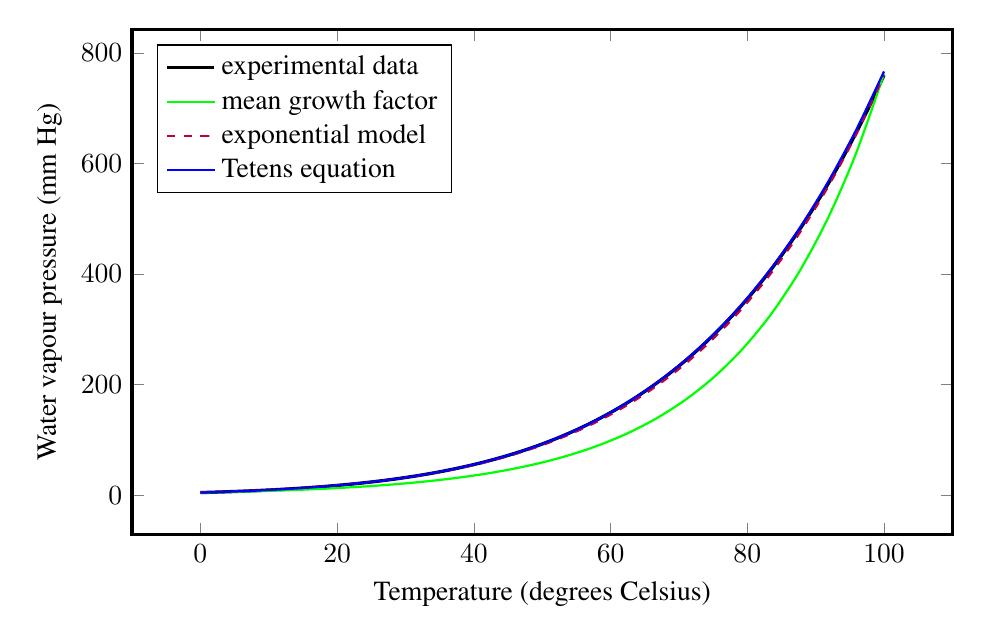
\begin{tikzpicture}
\tikzset{%%
  every mark/.append style={scale=1.0},%%
  scale=1.0%%
}
\pgfplotsset{%%
  every axis/.append style={font=\normalsize}%%
}
%%
\begin{axis}[%%
  axis line style=very thick,%%
  dotStyle/.style={very thick,black,mark=none},%%
  enlargelimits=true,%%
  height=8cm,%%
  legend cell align=left,%%
  legend pos=north west,%%
  plotStyle/.style={%%
    domain=0:100,%%
    mark=none,%%
    smooth,%%
    thick%%
  },%%
  width=12cm,%%
  %% x axis
  xlabel={\normalsize Temperature~(degrees~Celsius)},%%
  %% y axis
  ylabel={\normalsize Water vapour pressure~(mm~Hg)},%%
  scaled y ticks=false,%%
  y tick label style=/pgf/number format/fixed%%
]
%%
%%
\addplot[dotStyle] coordinates {
  (0, 4.579)
  (1, 4.926)
  (2, 5.294)
  (3, 5.685)
  (4, 6.101)
  (5, 6.543)
  (6, 7.013)
  (7, 7.513)
  (8, 8.045)
  (9, 8.609)
  (10, 9.209)
  (11, 9.844)
  (12, 10.518)
  (13, 11.231)
  (14, 11.987)
  (15, 12.788)
  (16, 13.634)
  (17, 14.53)
  (18, 15.477)
  (19, 16.477)
  (20, 17.535)
  (21, 18.65)
  (22, 19.827)
  (23, 21.068)
  (24, 22.387)
  (25, 23.756)
  (26, 25.209)
  (27, 26.739)
  (28, 28.349)
  (29, 30.043)
  (30, 31.824)
  (31, 33.695)
  (32, 35.663)
  (33, 37.729)
  (34, 39.898)
  (35, 42.175)
  (36, 44.563)
  (37, 47.067)
  (38, 49.692)
  (39, 52.442)
  (40, 55.324)
  (41, 58.34)
  (42, 61.5)
  (43, 64.8)
  (44, 68.26)
  (45, 71.88)
  (46, 75.65)
  (47, 79.6)
  (48, 83.71)
  (49, 88.02)
  (50, 92.51)
  (51, 97.2)
  (52, 102.09)
  (53, 107.2)
  (54, 112.51)
  (55, 118.04)
  (56, 123.8)
  (57, 129.82)
  (58, 136.08)
  (59, 142.6)
  (60, 149.38)
  (61, 156.43)
  (62, 163.77)
  (63, 171.38)
  (64, 179.31)
  (65, 187.54)
  (66, 196.09)
  (67, 204.96)
  (68, 214.17)
  (69, 223.73)
  (70, 233.7)
  (71, 243.9)
  (72, 254.6)
  (73, 265.7)
  (74, 277.2)
  (75, 289.1)
  (76, 301.4)
  (77, 314.1)
  (78, 327.3)
  (79, 341)
  (80, 355.1)
  (81, 369.7)
  (82, 384.9)
  (83, 400.6)
  (84, 416.8)
  (85, 433.6)
  (86, 450.9)
  (87, 468.7)
  (88, 487.1)
  (89, 506.1)
  (90, 525.76)
  (91, 546.05)
  (92, 566.99)
  (93, 588.6)
  (94, 610.9)
  (95, 633.9)
  (96, 657.62)
  (97, 682.07)
  (98, 707.27)
  (99, 733.24)
  (100, 760)
};
\addlegendentry{experimental data}
%%
%%
%% The mean growth factor model.
\addplot+ [plotStyle,green]
{4.579*(1.0525^x)};
\addlegendentry{mean growth factor}
%%
%%
%% The exponential model from Wikipedia.
\addplot+ [plotStyle,purple,dashed]
{exp(20.386 - (5132 / (273.15 + x)))};
\addlegendentry{exponential model}
%%
%%
%% The Tetens equation.
\addplot+ [plotStyle,blue]
{7.500638 * 0.61078 * exp((17.27*x) / (237.3 + x))};
\addlegendentry{Tetens equation}
\end{axis}
\end{tikzpicture}

\end{document}
